\chapter{\texorpdfstring{\ds and \dpl signal extraction}{Ds+ and D+ signal extraction}}

The main ingredient for the evaluation of the \ds/\dpl production-yield ratio is the \ds and \dpl raw yield, i.e., the number of reconstructed \ds and \dpl mesons. Due to the vast amount of combinatorial background and the limited efficiency of about 1\%, the extraction of the raw yield is not possible through a candidate counting method. Instead, the raw yield is obtained on a statistical basis by fitting the invariant-mass distribution of the \ds and \dpl candidates passing tight selection criteria. To reduce the combinatorial background and enhance the efficiency of D-meson selection, Machine Learning algorithms have been employed. The following sections describe the procedure for the extraction of the raw yield of \ds and \dpl mesons. 

\section{Machine Learning}
The term \emph{Machine Learning} (ML) is a broad and versatile concept, encompassing a wide range of algorithms that grant computers the capacity to learn and adapt without being explicitly programmed to do so~\cite{5392560}. A more comprehensive definition characterizes ML as the study of algorithms that enhance their performance (P) at a specific task (T) through the accumulation of experience (E)~\cite{mitchell1997machine}. In recent years, ML techniques have witnessed widespread adoption across diverse fields, with significant impacts realised especially with the emergence of generative models such as GPT~\cite{openai2023gpt4}.
ML algorithms have found extensive applications in the high-energy physics field, primarily for the task of distinguishing interesting signals from the vast background present in particle collision data. Furthermore, these algorithms have been employed as triggers, aiding in the rapid identification of events of interest, and have also been instrumental in event reconstruction. Notably, ML algorithms were used in the discovery of the Higgs boson~\cite{CMS:2012qbp}, one of the most significant achievements in the field of particle physics. \textcolor{red}{Aggiungere che permette di fare selezioni non lineari}

\subsection{Supervised learning}
Supervised learning is one of the main branches of machine-learning problems, together with unsupervised and reinforcement learning. Machine learning tasks are usually described in terms of how the machine learning system should process an example, which is a collection of features $\mathbf{x}$ that have been quantitatively measured from some object or event that one wants the machine learning system to process. In the case of supervised learning, each example is coupled with a corresponding label or target, $\mathbf{y}$. The objective of supervised learning is to learn to predict or infer $\mathbf{y}$ based on the associated features, $\mathbf{x}$.
Supervised learning problems exhibit further segmentation into two distinct sub-categories, known as classification and regression. In the former, the label $\mathbf{y}$ assumes values from a finite and discrete set of categories, often representing distinct classes or groups. In the latter, the label $\mathbf{y}$ takes the form of one or more continuous variables. This necessitates the learning system to deduce a continuous function or mapping between $\mathbf{x}$ and $\mathbf{y}$, where the goal is to predict and approximate numerical values rather than class affiliations.

The application of a supervised learning algorithm to a dataset involves the following steps: i. the model is trained on a set of labelled data, i.e., the value of $\mathbf{y}$ is known for each example in the training set; ii. the model is tested on a separate set of labelled data, known as the test set, to evaluate its performance; iii. the model is then used to make predictions on new, unseen data.

\subsubsection{Training}
During the training process, the model learns (i.e., adjusts its internal parameters) to map the input features $\mathbf{x}$ to the corresponding labels $\mathbf{y}$ by minimizing a loss function, which quantifies the discrepancy between the predicted and true labels. Typically used loss functions include the Mean Squared Error (MSE) for regression tasks and the Cross-Entropy loss for classification tasks. The loss function is minimized through an optimization algorithm, usually stochastic gradient descent~\cite{10.1214/aoms/1177729392}, which iteratively updates the model parameters to reduce the loss. Since an overoptimisation of the model on the training data can lead to poor generalization on unseen data (the model is said to be \emph{overfitting}), a regularisation term is often added to the loss function to penalize overly complex models. The training process continues until the model reaches a satisfactory level of performance on the training data, or until its performance does not improve further. 

Before the final model training, hyperparameters tuning is performed to optimize the model's performance. \emph{Hyperparameters} are parameters that are not learned during the training process, but rather define the model's architecture and the training process itself. Hyperparameters tuning is usually performed through a grid search or random search, where different combinations of hyperparameters are tested on a dedicated labelled dataset, different from the training set: the validation set. Models with different hyperparameter sets are trained with a reduced training phase, and those yielding the best performance are then selected for the final model training.

\subsubsection{Testing}
After the model has been trained, its performance is evaluated on a dataset that was not used during the training process, known as the test set. Like the training and validation sets, also the test set contains labelled examples. While during the training the model is optimised to minimise the loss function, the test set is used to estimate the model's generalization error, i.e., how well the model performs on unseen data. The model's performance is evaluated using metrics that are specific to the task at hand, such as accuracy for classification tasks, or Mean Squared Error (MSE) for regression tasks. Once the model achieves satisfactory performance on the test set, it is ready to be used for making predictions on unlabelled data.

\subsubsection{Cross-validation}

With the strategy defined above to optimise the hyperparameters, train the model and validate its performance, the dataset is divided into three subsets: the training set, the validation set, and the test set. When small datasets are involved, this division can lead to a suboptimal model, as the model's performance can be highly dependent on the specific examples in the training, validation, and test sets. Furthermore, this approach limits the amount of data available for training the model, which can lead to poor generalization. To mitigate this issue, a technique called cross-validation is often employed. It consists on dividing the training sample into $k$ subsets of equal size, called \emph{folds}. Then, the ML algorithm is trained $k$ times, each time using $k-1$ folds as training set, while the remaining fold is used as validation set. The model's performance is then averaged over the $k$ folds to obtain a more robust estimate of this quantity. This operation is repeated for each hyperparameter configuration to be considered. The hyperparameter configuration minimising the loss function is then chosen as the optimal configuration.

\section{\texorpdfstring{\ds and \dpl selection using Machine Learning}{Ds+ and D+ selection using Machine Learning}}

The task of extracting \ds and \dpl signals from the vast combinatorial background is a challenging one, due to the large amount of background compared to signal. It is however an excellent example of classification problem, and ML algorithms can therefore be exploited to enhance the efficiency of the selection. 

\subsection{Data preparation}
In order to train a ML model, a labelled dataset with a well defined set of features is required. The dataset is composed of signal and background examples. To obtain a pure sample of signal candidates, Monte Carlo simulations are used to generate \ds and \dpl mesons. Proton-proton collisions are generated using the \textsc{Pythia~8} event generator~\cite{Bierlich:2022pfr} with colour-reconnection Mode~2~\cite{Christiansen:2015yqa}, and the generated particles are propagated through the ALICE detector using the \textsc{Geant4} transport simulation toolkit~\cite{GEANT4:2002zbu}. To enrich the sample of heavy-flavour hadrons, $\mathrm{c\overline{c}}$ and $\mathrm{b\overline{b}}$ pairs are injected into each simulated event. 


%Due to the displaced topology of heavy-flavour decays and the continuous readout employed by the ALICE detector, the selection of events with charm or beauty hadrons produces ``fake'' vertices arising from the association of displaced decay tracks, affecting the reconstruction of heavy-flavour hadrons. To overcome this problem, minimum bias events are generated between charm or beauty enriched ones (\emph{gap-triggered} approach). Studies performed using different gap sizes have shown that a gap of 5 minimum bias events reduces the fake-vertex rate to an acceptable level, while keeping the simulation time reasonable. 

Only prompt and non-prompt \ds mesons are used to train the model, as \dpl mesons decay into the same final state as \ds mesons, and selections optimised to reconstruct \ds mesons are also effective for \dpl mesons. 

Background candidates are obtained from real data, as MC simulations may not able to reproduce the complexity of soft processes occurring in the underlying event, or may not be able to model the detector response accurately. The background examples are obtained by selecting candidates from a subsample of the full data sample (correspondig to its 3\%) in an invariant-mass region away from both the \ds and \dpl mass peaks, where $1.7 < M < 1.75$~\gevcc or \mbox{$2.1 < M < 2.15$~\gevcc}, as shown in Fig.~\ref{fig:ml_training_mass}. 

\begin{figure}[htb]
    \centering
    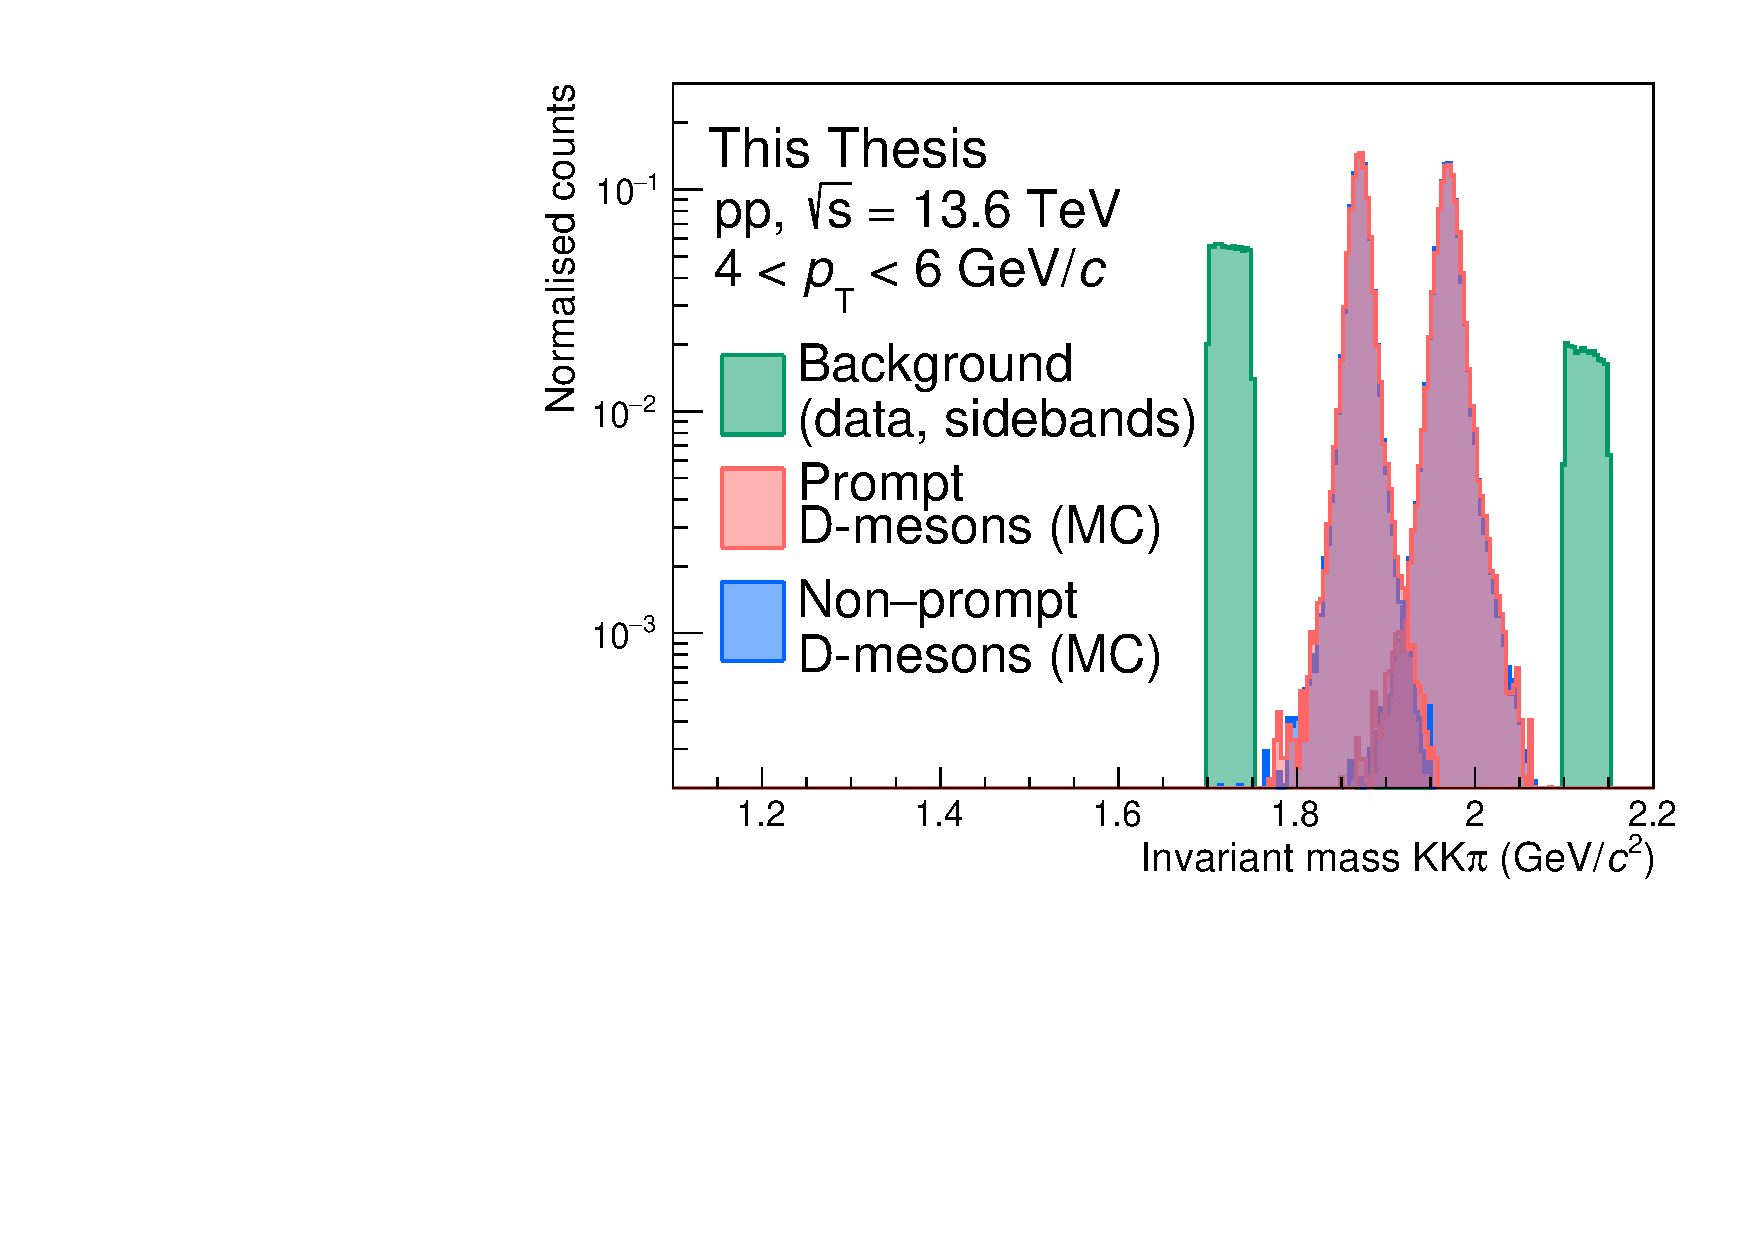
\includegraphics[width=0.7\textwidth]{Figures/Chapter 5/Mass.pdf}
    \caption{Invariant mass distribution of the backgound candidates used to train the ML model (green) and of prompt and non-prompt D-mesons (blue and orange, respectively), taken from Monte Carlo simulations, in the $4<\pt<6$~\gevc interval. Background candidates are selected in the $1.7 < M < 1.75$~\gevcc or \mbox{$2.1 < M < 2.15$~\gevcc} invariant-mass interval.}
    \label{fig:ml_training_mass}
\end{figure}

The dataset is then divided into two different subsamples. The first comprehends 80\% of the data, and is used to train the model, while the remaining 20\% is used to test its performance. In addition, since the D-mesons decay topology can significantly differ depending on the \pt of the meson due to different Lorentz boosts, the dataset is divided into several \pt intervals, and the model is trained and tested separately for each of them. The total number of candidates availabe for training and testing the model is reported in Table~\ref{tab:training_sample} for the considered \pt intervals.


\begin{table}[htb]
    \begin{center}
    \begin{tabular}{c|ccc}
         \toprule
         \pt (\gevc) & Prompt \ds & Non-prompt \ds & Background\\
         \midrule         
         0--1.5     & $\sim 4.6 \times 10^{3}$  & $\sim 21  \times 10^{3}$   & $\sim 726  \times 10^{3}$ \\
         1.5--2     & $\sim 6.1 \times 10^{3}$  & $\sim 24  \times 10^{3}$   & $\sim 92   \times 10^{3}$\\
         2--3       & $\sim 26  \times 10^{3}$  & $\sim 96  \times 10^{3}$   & $\sim 123  \times 10^{3}$ \\
         3--4       & $\sim 34  \times 10^{3}$  & $\sim 124 \times 10^{3}$   & $\sim 114  \times 10^{3}$ \\
         4--5       & $\sim 31  \times 10^{3}$  & $\sim 113 \times 10^{3}$   & $\sim 63   \times 10^{3}$\\
         5--6       & $\sim 24  \times 10^{3}$  & $\sim 89  \times 10^{3}$   & $\sim 29   \times 10^{3}$\\
         6--8       & $\sim 32  \times 10^{3}$  & $\sim 115 \times 10^{3}$   & $\sim 22   \times 10^{3}$\\
         8--12      & $\sim 23  \times 10^{3}$  & $\sim 89  \times 10^{3}$   & $\sim 10   \times 10^{3}$\\
         12--24     & $\sim 9.7 \times 10^{3}$  & $\sim 39  \times 10^{3}$   & $\sim 2.6  \times 10^{3}$ \\
         \bottomrule
    \end{tabular}
    \caption{Number of candidates within the \pt intervals used to train and test the model.}
    \label{tab:training_sample}
    \end{center}
\end{table}

\begin{sloppypar}
To produce a balanced dataset, the number of candidates in each class is equalised to the number of examples in the minority class. This is achieved by randomly selecting a subset of the majority classes. The balanced dataset is then used to train the model.
\end{sloppypar}

The choice of features used to separate signal from background is crucial, as they must be able to discriminate between signal and background candidates, and must be chosen in such a way that no bias is introduced in the final result. The variables used to train the model were introduced in Chapter~\ref{chap:reconstruction}, and are a mix of topological, kinematic, and PID variables. The key idea is to exploit the displaced topology of the D-meson decay, which is a distinctive feature of the signal candidates, the kinematic properties of the D-meson decay, and the PID information of the daughter tracks to discriminate between signal and background candidates. The features used to train the model are reported in Table~\ref{tab:ml_training_vars}. The number in parenthesis after $n\sigma$ indicates the prong number.

\begin{table}[htb]
    \begin{center}
    \begin{tabular}{c}
         \toprule
         Variable\\
         \midrule         
         cos$\theta_{p}$\\
         cos$\theta_{p}^{xy}$\\
         Decay length\\
         Decay length XY\\
         Candidate impact parameter XY\\
         $\lvert \cos^{3}\theta'(\mathrm K)\rvert$\\
         Prong 0 impact parameter XY\\
         Prong 1 impact parameter XY\\
         Prong 2 impact parameter XY\\
         $n\sigma_{\mathrm comb}^{\pi}(0)$\\         
         $n\sigma_{\mathrm comb}^{\pi}(1)$\\
         $n\sigma_{\mathrm comb}^{\pi}(2)$\\
         $n\sigma_{\mathrm comb}^{\mathrm K}(0)$\\
         $n\sigma_{\mathrm comb}^{\mathrm K}(1)$\\
         $n\sigma_{\mathrm comb}^{\mathrm K}(2)$\\
         \bottomrule
    \end{tabular}
    \caption{Candidate features used to train the ML model.}
    \label{tab:ml_training_vars}
    \end{center}
\end{table}

The invariant mass of the candidate and its \pt are not used to train the model. Exploiting such variables would introduce a bias in the final result, as the model would be trained to select candidates within a specific invariant mass region (that of \ds and \dpl mesons) or \pt. This would affect both the selection of the candidates and the \pt distribution of the final sample, leading to a biased \pt-differential yield. However, some of the variables used to train the model may be correlated with the invariant mass of the candidate, and the ML may learn to discriminate the signal from the background by exploiting the correlation with the \ds meson mass and transverse momentum, rather than the physical properties of the signal and background. To exclude this possibility, the correlation between the features used to train the model is studied. To quantitatively describe the correlation between the variables, the Pearson correlation coefficient $\rho$ is evaluated for each pair of variables. It is defined as the ratio between the covariance of two variables and the product of their standard deviations, $\rho(x,y) = \mathrm{cov}(x,y)/(\sigma_{x}\sigma_{y})$. It expresses the strength and direction of a linear correlation between two variables, ranging from $\rho = 1$ (perfect positive linear correlation) to $\rho = -1$ (perfect negative linear relationship). $\rho = 0$ indicates no linear correlation.

The correlation matrix of the features used to train the model is shown in Fig.~\ref{fig:ml_training_vars} for the prompt \ds, non-prompt \ds and background classes, in the $2<\pt<3$~\gevc. The correlation with the invariant mass and the transverse momentum is also reported. The Pearson coefficient is encoded in the colour of the cell, with red indicating a positive correlation, blue a negative correlation, and grey no correlation. The correlation matrix shows that the variables used to train the model are not correlated with the invariant mass of the candidate, suggesting that a ML should not modify the invariant-mass distribution of the selected candidates, which would introduce a bias in the measurement.

Variables carrying the same physical information, such as those related to the candidate decay length, pointing angle, and impact parameter, are strongly correlated among each other, as expected. Different degrees of correlation between the same variables in the different classes are observed. The ML model can exploit these differences to discriminate between signal and background candidates.

\begin{figure}[htb]
    \centering
    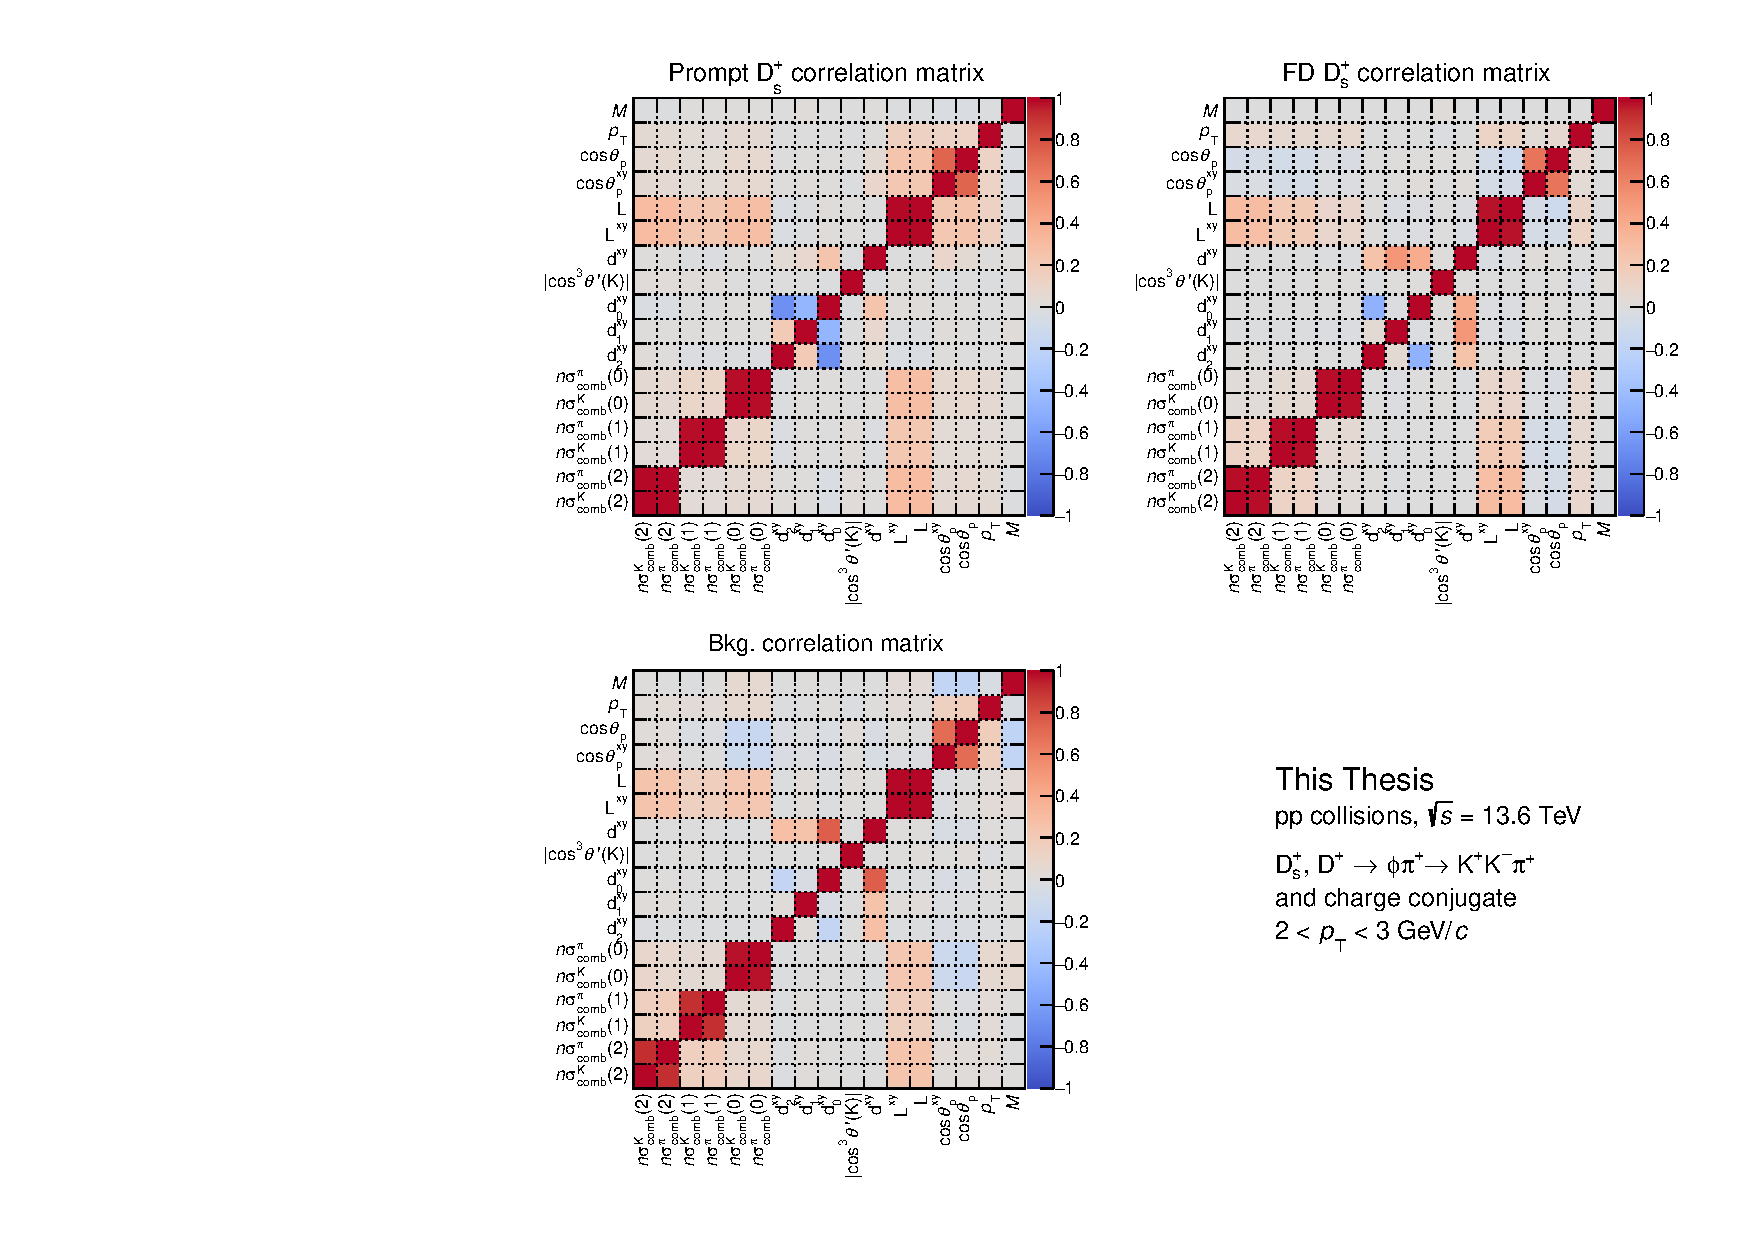
\includegraphics[width=\textwidth]{Figures/Chapter 5/CorrelationMatrix.pdf}
    \caption{Distribution of the candidate variables used to train the ML model.}
    \label{fig:ml_training_vars}
\end{figure}

\subsection{Boosted Decision Trees}
Once the training dataset has been composed, and the features have been selected, the ML algorithm has to be chosen. Several algorithms are available, each with its own strengths and weaknesses. The choice of the algorithm depends on the specific problem to solve, the size of the dataset, and the computational resources available. In this work, the XGBoost~\cite{DBLP:xgboost} Boosted Decision Trees (BDT) algorithm is used. It has achieved state-of-the-art results in a number of machine learning and data mining challenges (for example in Ref.~\cite{kaggle:higgs}). In addition, this algorithm, which is available as a open-source package, can be easily parallelised on CPUs and GPUs~\cite{mitchell2017accelerating} reducing the training and application time.

BDT is a powerful and versatile algorithm that has been widely used in high-energy physics for a variety of tasks, such as event classification, regression, and anomaly detection. The BDT algorithm is based on the concept of decision trees, which are a type of supervised learning algorithm that can be used for both classification and regression tasks. A decision tree is a flowchart-like structure in which each internal node represents a feature or attribute, each branch represents a decision rule, and each leaf node represents the outcome. The tree is constructed by recursively splitting the dataset into subsets based on the value of a feature that results in the best separation between the classes. The splitting process continues until a stopping criterion is met, such as a maximum tree depth or a minimum number of samples in a leaf node.
